\chapter{Entropy and Randomness}\label{sec:Entropy and randomness}

In its most general form, a data sequence can be considered as a realization of a stochastic process. A stochastic process is usually described as either a sequence of random variables (ie a set of $(X_t)_{t \geq 0} : \omega \rightarrow X_t({\omega})$), or a single random variable over the space of functions (ie $X : \omega \rightarrow X(\omega) = X_{\omega} = \{ t \rightarrow X_{\omega}(t) \}$.

As we wish to measure -somehow- the degree of "randomness" of a data sequence, we will find more convenient to use the former view (ie consider a data sequence as a countable sequence of random variables), as it allows to use the framework of information theory.

First, we will recall the basic definitions of information theory : entropy, relative entropy (ie KL divergence), conditional entropy and mutual information. Then we will write some results regarding the application of \gls{it} to data sequence. Last, we will describe two of the most used empirical measurements : \gls{apen} and \gls{sampen}.

The basic of \gls{it} are introduced in \cite{bishop_pattern_2016}, \cite{ProbabilisticGraphicalModels}, and \cite{ProbabilisticMachineLearning}. One of the reference books on the subject is \cite{cover_elements_2006}, and goes much further than the scope of this report. Of course, the interested reader will also refer to the seminal paper by Shannon : \cite{shannon_mathematical_1948}.

\textbf{Entropy} : given a random variable $X$, either discrete or continuous, taking values in a measurable space $\mathcal{X}$, and its probability distribution $p$, the amount of information given by a given realization $x$ is given by $\log{\frac{1}{p(x)}} = - \log{p(x)}$ (the lower the probability, the higher the amount of information). 

The average amount of information (over all possible values of $x$) required to describe the random variable $X$ is the entropy of $X$ : 
\begin{align}
    \mathcal{H}(X) = - \sum_{x \in \mathcal{X}} p(x)\log{p(x)}
\end{align}
(or $-\int_{\mathcal{X}} p(x)\log{p(x)}dx$).

\textbf{Relative entropy, KL divergence} : when approximating the true data distribution $p$ by a distribution $q$, we require in average a quantity of information $-\sum_{x \in \mathcal{X}} p(x) \log{q(x)} $ to describe $X$. The difference between the optimal amount of information (ie the entropy $\mathcal{H}(X)$) and this quantity is the well-known relative entropy, of KL-divergence between $p$ and $q$ :
\begin{align}
    \mathbb{KL}(p \vert\vert q) &= \sum_{x \in \mathcal{X}} p(x) \log{\frac{p(x)}{q(x)}} \\
    &= \int_\mathcal{X} p(x) \log{\frac{p(x)}{q(x)}}dx
\end{align}
The properties of KL-divergence (positiveness, non symmetry) are well described in the sources above.

\textbf{Conditional Entropy} : we now consider two random variables $X$ and $Y$, and wish to measure the degree of relationship between them. We define the conditional entropy of, for example, $Y$ given $X$, as the amount of information we get observing the values of $Y$ given $X$, averaged over the joint probability. Formally :
\begin{align*}
    \mathcal{H}(Y \vert X) &= -\sum_{x,y \in \mathcal{X, Y}} p(x,y) \log{p(y \vert x}) \\
    &= - \int_{\mathcal{X,Y}} p(x,y) \log{p(y\vert x}) \, dxdy
\end{align*}
By basic calculation, we get $\mathcal{H}(X,Y) = \mathcal{H}(Y\vert X) + \mathcal{H}(X) =  \mathcal{H}(X\vert Y) + \mathcal{H}(Y)$

\textbf{Mutual Information} - last, still considering two random variables $X, Y$, the mutual information is the additional amount of information we need to describe $X,Y$ when we assume independence (ie use $p(x)p(y)$) rather than use the true joint probability $p(x,y)$. This amount is $- \log{p(x)p(y)} - (-\log{p(x,y)}) = \log{\frac{p(x,y)}{p(x)p(y)}} $, that we average over the true distribution $p(x,y)$:
\begin{align}
    \mathcal{I}(X,Y) &= \sum_{x,y \in \mathcal{X,Y}} p(x,y) \log{\frac{p(x,y)}{p(x)p(y)}}
\end{align}

The relationships between entropy, relative entropy, conditional entropy and mutual information, are well described using a Venn diagram:

\begin{figure}[h]
\begin{centering}
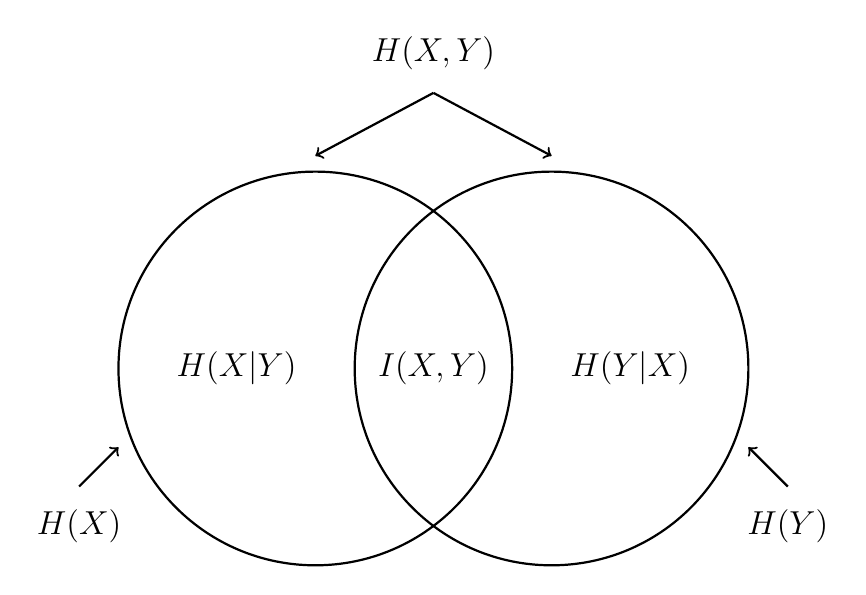
\begin{tikzpicture}
  % Define sets
  \def\radius{2.5}
  \def\dx{3.0}

  % Draw the circles
  \draw[thick] (0,0) circle(\radius); % H(X)
  \draw[thick] (\dx,0) circle(\radius); % H(Y)

  % Labels inside the circles
  \node at (-1.0,0) {\large $H(X|Y)$};
  \node at (4.0,0) {\large $H(Y|X)$};
  \node at (1.5,0) {\large $I(X,Y)$};

  % Arrows and labels outside
  \draw[->, thick] (-3.0,-1.5) -- (-2.5,-1.0);
  \node at (-3.0,-2.0) {\large $H(X)$};

  \draw[->, thick] (6.0,-1.5) -- (5.5,-1.0);
  \node at (6.0,-2.0) {\large $H(Y)$};

  \draw[->, thick] (1.5, 3.5) -- (0.0, 2.7);
  \draw[->, thick] (1.5, 3.5) -- (3.0, 2.7);
  \node at (1.5,4.0) {\large $H(X,Y)$};

\end{tikzpicture}
\end{centering}
\end{figure}

For example : $\mathcal{I}(X,Y) = \mathcal{H}(X) + \mathcal{H}(Y) - \mathcal{H}(X,Y)$, etc.

If we now consider a sequence of $n$ random variables, a way to describe the randomness of the sequence is to measure how the entropy of the joint distribution grow with $n$. (see \cite{cover_elements_2006} p63). Typically, if the random variables are independent, we can expect the entropy to grow at each step $n$ by the full amount of $\mathcal{H}(X_n)$. On the other hand, if correlations exist, then we can expect the overall entropy to grow by a lesser amount.

Formally, the \textbf{entropy rate} of a stochastic process $(X_n)_{n \in \mathbb{N}^*}$ is defined by:
\begin{align}
    \label{entropy_rate}
    \mathcal{H}(X) &= \underset{n \rightarrow \infty}{\lim} \frac{1}{n} \mathcal{H}(X_1, X_2, ..., X_n) 
\end{align}
\textit{when the limit exists}. This is the entropy per symbol.

\cite{cover_elements_2006} also defines a \textbf{conditional entropy rate}
\begin{align}
    \label{cond_entropy_rate}
    \mathcal{H}'(X) &= \underset{n \rightarrow \infty}{\lim} \frac{1}{n} \mathcal{H}(X_n \vert X_{n-1},...X_2, X_1)
\end{align}
when the limit exists. This is the entropy of the latest random variable, given the past realizations.

An important result is that, when $(X_n)$ is stationary, both limits exist and are equal.

The question naturally arises that, given a data sequence, how do we compute an approximation of \ref{entropy_rate} or \ref{cond_entropy_rate}. We now introduce the \gls{apen} and \gls{sampen} (see \cite{delgado-bonal_approximate_2019} and \cite{pincus_approximate_1991}).

\textbf{Approximate Entropy} - Approximate Entropy is a measure of the log probability that patterns, that were identified in the data through the examination of sub sequences of a given length, still remain when considering longer subsequences. 

Formally, let $x = (x_1,x_2,...,x_N)$ be a data sequence of length $N$, $m$ an integer ($0 < m \leq N)$, and $r>0$ a measure of acceptable noise. We define as \textit{blocks} of length $m$ the subsequences $b_i^m = \{x_i, x_{i+1},...,x_{i+m-1}\}$, starting at $i$ with $(1 \leq i \leq N-m+1)$. For two blocks $b_i^m$ and $b_j^m$, we define a component-wise distance $d_{ij}^m = \underset{k=0,1,..,m-1}{\max}\vert b_{i+k}^m - b_{j+k}^m\vert$. We consider "close enough" (ie similar) those blocks whose distance is lower than the acceptable noise (tolerance) $r$, and calculate the frequency of those similar blocks ($b_i^m, b_j^m$) w.r.t. all blocks of length $m$ for a given $b_i^m$ : 
\begin{align}
    \label{Cim}
    C_i^m(r) = \frac{\text{number of $j \leq N-m+1$ s.t. $d_{ij} \leq r$}}{\text{number of blocks of length $m$ : $N-m+1$}}
\end{align}
We then average the $\log{C_i^m}$ over all possible subsequences $b_i$ :
\begin{align*}
    \Phi^m(r) &= \frac{1}{N-m+1} \sum_{i=1}^{N-m+1} \log{C_i^m(r)}
\end{align*}
We can see $\Phi^m(r)$ as the average of the log probability of two subsequences of length $m$ to be similar (up to the tolerance $r$).
Finally, we compute:
\begin{align}
    \text{ApEn}(m,r,N) &= \Phi^m(r) - \Phi^{m+1}(r)
\end{align}
When $m \ll N$, then $-\text{ApEn}(m,r,N) \sim \frac{1}{N+1}\sum_{i=1}^{N+1} \log{\frac{C_i^{m+1}}{C_i^m}}$, which is the average over $i$ of the log of the conditional probability of two sequences $b_i^{m+1}, b_j^{m+1}$ of length $m+1$ be similar given that they are already similar for lengths $1,2,...,m$.

Last, $\text{ApEn}(m,r,N)$ is a statistical estimator of:
\begin{align}
    \text{ApEn}(m,r) &= \underset{N \rightarrow \infty}{\lim} \text{ApEn}(m,r,N)
\end{align}
Intuitively, the greater the regularity in a data sequence, the greater the likelihood that patterns existing for subsequences of length $m$ still remain for subsequences of greater length, ie the smaller $\text{ApEn}$, and conversely.

Key properties of $\text{ApEn}$ include:
\begin{itemize}
    \item $\text{ApEn}$ is independent of any model of the data sequence.
    \item due to its construction, $\text{ApEn}$ is non-negative, is finite for stochastic processes and deterministic processes with noise.
    \item following \cite{pincus_approximate_1991}, it is imperative to eliminate any trend in the data sequence before computing $\text{ApEn}$ and drawing conclusions.
    \item typical recommended values for $m$ are 2 and 3. Typical recommended values for $r$ are in the range of 0.1 to 0.25 the standard deviation of the data sequence, in order to allow a sufficient number of subsequences close within a distance $r$, and reasonable estimates of the conditional probabilities.
    \item if the noise is significant (ie signal-to-noise ratio lower than three), then precautions must be taken with the interpretation of $\text{ApEn}$.
    \item Regular measurements of the data sequence over time are required.
    \item Normalization of data sequences is required before computations of $\text{ApEn}$ to compare data sequences between each other.
\end{itemize}

\textbf{Sample Entropy} - we can see in \ref{Cim} that a given subsequence $b_i^m$ is counted in both the numerator and the denominator. If this ensures numerical stability (ie no attempt to calculate $\log{0}$ for example), this also introduces a bias in the calculation of the probability estimates. $\text{SampEn}$ explicitly discounts the subsequence $b_i^m$ from the calculations to remove the bias.

Formally:
\begin{align}
    A_i^m(r) &= \frac{1}{N-m-1} \{ \text{number of blocks $b_j^{m+1}$  of length $m+1$ s.t. $i \neq j$ and $d_{ij}^{m+1} \leq r$} \} \\
    B_i^m(r) &= \frac{1}{N-m} \{\text{number of blocks $b_j^m$ of length $m$ s.t. $i \neq j$ and $d_{ij}^m \leq r$} \} \\
    B^m(r) &= \frac{1}{N-m} \sum_{i=1}^{N-m} B_i^m(r) \\
    A^m(r) &= \frac{1}{N-m-1} \sum_{i=1}^{N-m-1} A_i^m(r)
\end{align}
And
\begin{align}
    \text{SampEn}(m,r,N) &= -\log{\frac{A^m(r)}{B^m(r)}} \\
    \text{SampEn}(m,r) &= - \underset{n \rightarrow \infty}{\lim } \log{\frac{A^m(r)}{B^m(r)}}
\end{align}

% I want to do a footnote right here \footnote{this is my first footnote}